\documentclass[a4paper,11pt]{article}

\usepackage[utf8]{inputenc}

\usepackage{graphicx}
\usepackage{caption}
\usepackage{subcaption}

\usepackage{hyperref}

\usepackage{pgfplots}
\pgfplotsset{compat=1.18} 

\usepackage{minted}

\begin{document}

\title{
    \textbf{Assignment 8 Report - Trees in Java}
}
\author{Dean Tsankov}
\date{\today}

\maketitle

\section*{Introduction}

In this assignment I will present an implementation of a binary tree data structure, its initialization, add element and search for element functionalities, achieved using recursive calls, an alternative non recursive implementation of the add, and finally I will use an explicit stack to show the traversal of the tree instead of relying on the inbuilt stack. 
\\

First off, let us introduce what a tree is. This data structures builds upon our understanding of the linked list type structures. In a tree there is a single root element from which( in the case of a binary tree) up to two branches containing two other elements emerge. Each of these branches could also have its own up to two branches and so on. When a branch. or also called a Node, does not have even a single other element connected to it, it is referred to as a leaf. 
\\

For a binary tree it is also important to mention that by the definition the structure is supposed to be ordered. As such we will know that each left branch has a value less than its parent node and a right branch has a larger value than the parent. While this might introduce some amount of complexity to adding elements, since we would have to place them in the exact right spot, having an ordered structure greatly reduces lookup times.

\section*{The binary tree}

To construct a binary tree, as explained we need to have an underlying {\tt Node} class with a value, a left
branch and a right branch reference. The value will be of a generic type, to allow us flexibility in using this structure.
When thinking about sorted trees there is a requirement for the value of each node to be somehow comparable. i.e. it should extend the {\tt Comparable} abstract class. The tree itself only holds the reference to the root element of the tree. Most of this part of the code is provided so we move on to the methods of the structure.

\subsection*{Add}

\begin{minted}[
frame=single,
framesep=2mm,
baselinestretch=1.2,
fontsize=\footnotesize,
]{java}
    (...)
    public void add(T value) {
        if (root == null) {
            root = new Node(value);
        }else{
            addRec(value, root);
        }
    }
    (...)
\end{minted}

For our recursive {\tt add} method, we need to first begin the function call by a helper function which does not require a node parameter but simply passes the root as the inital point of traversal.

\begin{minted}[
frame=single,
framesep=2mm,
baselinestretch=1.2,
fontsize=\footnotesize,
]{java}
    (...)
    private void addRec(T value, Node itr) {
        if (itr.value != value) {
            if (itr.value.compareTo(value) > 0) {
                if (itr.left != null) {
                    addRec(value, itr.left);
                    return;
                } else {
                    itr.left = new Node(value);
                    return;
                }
            } else {
                if (itr.right != null) {
                    addRec(value, itr.right);
                    return;
                } else {
                    itr.right = new Node(value);
                    return;
                }
            }
        }
    }
    (...)
\end{minted}

The main add method works in the following way. Firstly we check if the value is already in the tree if so, nothing happens if not we proceed to the actual logic. Depending on whether the value we want to add is more or less then that of the current node we go to the left or right branch of the sub-tree respectively. Unless there is none (there is a null reference) in which case we know that is the place to add the new element. Here important to note is that since we are working with the generic type we cannot simply us the comparison operators {\tt </>}, but instead have to rely on the {\tt.compareTo()} function a comparable type is required to have. 
\\

Bellow is a benchmark-ed execution of the add operation in an increasing amount of random elements in the tree. Thinking about the way the algorithm always splits its work in two as it goes down the tree, we would expect an {\tt O(logn)} complexity. Which is closely followed by the graph (both axes are logarithmicaly mapped)

\begin{figure}[H]
    \centering
    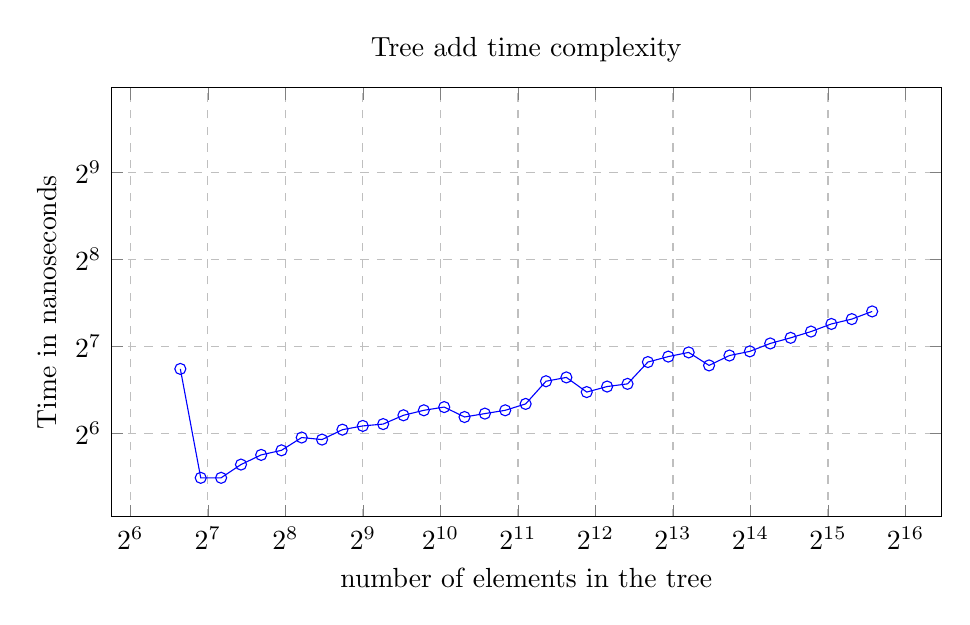
\begin{tikzpicture}
        \begin{axis}[
            title={Tree add time complexity},
            width=\linewidth,
            height=200,
            xlabel={number of elements in the tree},
            ylabel={Time in nanoseconds},
            ymin=0, ymax=1000,
            xmode=log,
            log basis x={2},
            ymode=log,
            log basis y={2},
            ymajorgrids=true,
            xmajorgrids=true,
            grid style=dashed,
        ]
        

        \addplot[
            color=blue,
            mark=o,
            ]
            coordinates {
            (100,107)(120,45)(144,45)(172,50)(206,54)(247,56)(296,62)(355,61)(426,66)(511,68)(613,69)(735,74)(882,77)(1058,79)(1269,73)(1522,75)(1826,77)(2191,81)(2629,97)(3154,100)(3784,89)(4540,93)(5448,95)(6537,113)(7844,118)(9412,122)(11294,110)(13552,119)(16262,123)(19514,131)(23416,137)(28099,144)(33718,153)(40461,159)(48553,169)
            };
            
            
        \end{axis}
        \end{tikzpicture}
    \caption{Tree add time complexity}
    \label{fig:plot1}
\end{figure}

\subsubsection*{Non recursive add}
Here I would also like to present a non-recursive way of performing an add to the tree, the logic is the same, except instead of the recursive calls we use a while loop to iterate through the nodes we require to find the correct position.

\begin{minted}[
frame=single,
framesep=2mm,
baselinestretch=1.2,
fontsize=\footnotesize,
]{java}
    (...)
    public void addNonRec(T value) {
        if (root == null) {
            root = new Node(value);
        } else {
            Node itr = root;
            Node prev = null;
            boolean isLess = false;
            while (itr != null) {
                prev = itr;
                if (value.compareTo(itr.value) < 0) {
                    itr = itr.left;
                    isLess = true;
                } else {
                    itr = itr.right;
                    isLess = false;
                }
            }
            if (isLess) {
                prev.left = new Node(value);
            } else {
                prev.right = new Node(value);
            }
        }
    }
    (...)
\end{minted}

It is not the cleanest implementation of the concept but it does work, and was actually the first of the two add versions I wrote, since it was a bit easier to think in terms of looping through the nodes instead of splitting function calls and traversing that way. In any case the graph bellow shows that both implementations are about as even in terms of execution time, and as such which one we choose is a matter of either personal preference or tertiary considerations.

\begin{figure}[H]
    \centering
    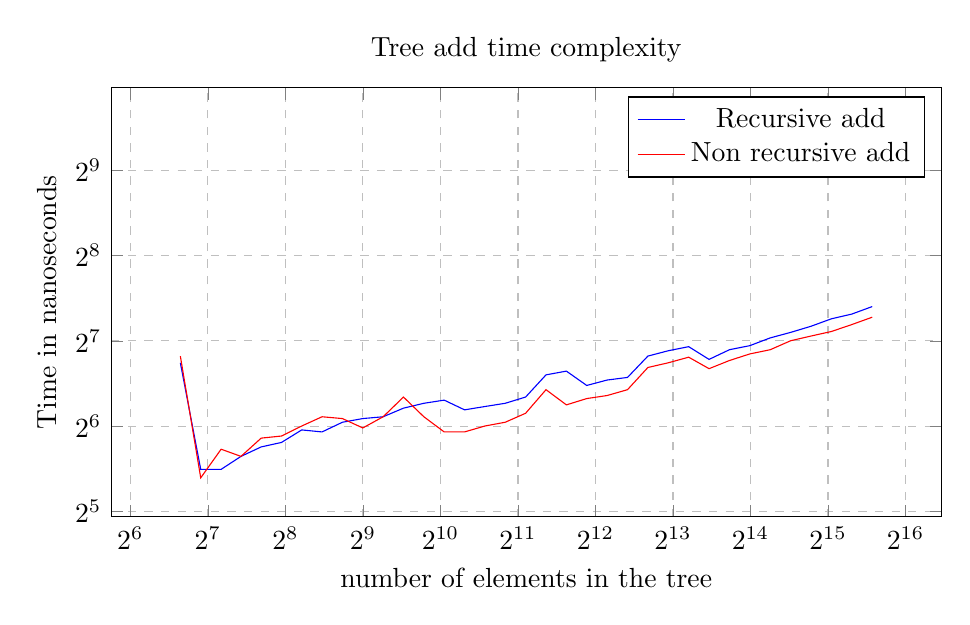
\begin{tikzpicture}
        \begin{axis}[
            title={Tree add time complexity},
            width=\linewidth,
            height=200,
            xlabel={number of elements in the tree},
            ylabel={Time in nanoseconds},
            ymin=0, ymax=1000,
            xmode=log,
            log basis x={2},
            ymode=log,
            log basis y={2},
            ymajorgrids=true,
            xmajorgrids=true,
            grid style=dashed,
        ]
        

        \addplot[
            color=blue,
            ]
            coordinates {
            (100,107)(120,45)(144,45)(172,50)(206,54)(247,56)(296,62)(355,61)(426,66)(511,68)(613,69)(735,74)(882,77)(1058,79)(1269,73)(1522,75)(1826,77)(2191,81)(2629,97)(3154,100)(3784,89)(4540,93)(5448,95)(6537,113)(7844,118)(9412,122)(11294,110)(13552,119)(16262,123)(19514,131)(23416,137)(28099,144)(33718,153)(40461,159)(48553,169)
            };
            \addlegendentry{Recursive add}
            
        \addplot[
            color=red,
            ]
            coordinates {
            (100,113)(120,42)(144,53)(172,50)(206,58)(247,59)(296,64)(355,69)(426,68)(511,63)(613,69)(735,81)(882,69)(1058,61)(1269,61)(1522,64)(1826,66)(2191,71)(2629,86)(3154,76)(3784,80)(4540,82)(5448,86)(6537,103)(7844,107)(9412,112)(11294,102)(13552,109)(16262,115)(19514,119)(23416,128)(28099,133)(33718,138)(40461,146)(48553,155)
            };   
            \addlegendentry{Non recursive add}
        \end{axis}
        \end{tikzpicture}
    \caption{Tree add time complexity}
    \label{fig:plot1}
\end{figure}

\subsection*{Lookup}

Next we continue with the search for an element function:

\begin{minted}[
frame=single,
framesep=2mm,
baselinestretch=1.2,
fontsize=\footnotesize,
]{java}
    (...)
    public boolean lookup(T key) {
        return lookupRec(key, root);
    }

    private boolean lookupRec(T key, Node itr) {
        if (itr.value != key) {
            if (itr.value.compareTo(key) > 0) {
                if (itr.left != null) {
                    return lookupRec(key, itr.left);
                } else {
                    return false;
                }
            } else {
                if (itr.right != null) {
                    return lookupRec(key, itr.right);
                } else {
                    return false;
                }
            }
        } else {
            return true;
        }
    }
    (...)
\end{minted}

In actuality the search function over the tree works in much the same way as the adding, since we are going through the elements comparing the value with branches in depth. The difference here is that if we in fact find a match we return true and if not - false, instead of adding. For the recursive algorithm to work there is again a helper initial call function. 

\subsubsection*{Binary search comparison}

Again, since the algorithm is so similar to the add method the time complexity should also follow a general {\tt O(logn)} complexity. Moreover if we think about what we do here it is essentially the same procedure as with the binary search implemented in a previous assignment. In order to facilitate this I ran benchmarks on both and the results are coherent.


\begin{figure}[H]
    \centering
    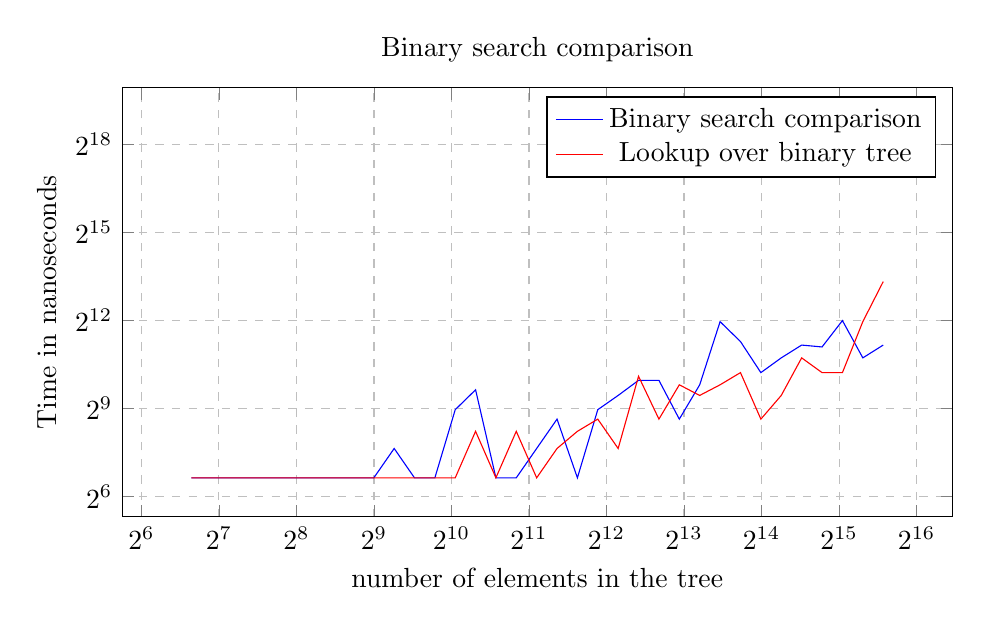
\begin{tikzpicture}
        \begin{axis}[
            title={Binary search comparison},
            width=\linewidth,
            height=200,
            xlabel={number of elements in the tree},
            ylabel={Time in nanoseconds},
            ymin=0, ymax=1000000,
            xmode=log,
            log basis x={2},
            ymode=log,
            log basis y={2},
            ymajorgrids=true,
            xmajorgrids=true,
            grid style=dashed,
        ]
        

        \addplot[
            color=blue,
            ]
            coordinates {
            (100,100)(120,100)(144,100)(172,100)(206,100)(247,100)(296,100)(355,100)(426,100)(511,100)(613,200)(735,100)(882,100)(1058,500)(1269,800)(1522,100)(1826,100)(2191,200)(2629,400)(3154,100)(3784,500)(4540,700)(5448,1000)(6537,1000)(7844,400)(9412,900)(11294,4000)(13552,2500)(16262,1200)(19514,1700)(23416,2300)(28099,2200)(33718,4100)(40461,1700)(48553,2300)
            };
            \addlegendentry{Binary search comparison}

        \addplot[
            color=red,
            ]
            coordinates {
            (100,100)(120,100)(144,100)(172,100)(206,100)(247,100)(296,100)(355,100)(426,100)(511,100)(613,100)(735,100)(882,100)(1058,100)(1269,300)(1522,100)(1826,300)(2191,100)(2629,200)(3154,300)(3784,400)(4540,200)(5448,1100)(6537,400)(7844,900)(9412,700)(11294,900)(13552,1200)(16262,400)(19514,700)(23416,1700)(28099,1200)(33718,1200)(40461,4000)(48553,10300)
            };
            \addlegendentry{Lookup over binary tree}
            
            
        \end{axis}
        \end{tikzpicture}
    \caption{Tree add time complexity}
    \label{fig:plot1}
\end{figure}

\subsection*{Depth first traversal and the explicit stack}

In the assignment outline we are provided a very simple yet very functional way to traverse the tree in way of its order i.e. a print method which yields a sorted sequence. This function uses a depth first methodology, that is it goes as deep into the tree as possible and on its way back returns the required information. What is not so explicit about the function is that it ultimately relies on the general program execution stack. It pushes operations onto it as it goes in depth into the tree, and later pops (executes) them in an ordered manner. 
\\

I will here show an explicit way to perform this using my dynamic stack structure from some assignments ago.

\begin{minted}[
frame=single,
framesep=2mm,
baselinestretch=1.2,
fontsize=\footnotesize,
]{java}
    (...)
    public void printExplStack() {
        DynamicStack<Node> stk = new DynamicStack<Node>();
        Node itr = this.root;
        
        while (itr.left != null && itr != null) {
            stk.push(itr);
            itr = itr.left;
        }

        while(itr != null) {
            System.out.println(itr.value);
            if (itr.right != null) {
                itr = itr.right;
                stk.push(itr);
                while (itr.left != null) {
                    itr = itr.left;
                    stk.push(itr);
                }
            }
            itr = stk.pop();
        }
    }
    (...)
\end{minted}

With this function our plan is as follows. We go to the left most element and push the elements we traversed along the way on the explicit stack. After this we begin a loop which assumes that all of the elements to the left of the given (current) one have been printed and those to the right have not. We print the element itself and check whether it has right branches, if it does then we go to the right one and again from there try to reach the left most element while pushing the trace into the stack. If there was no reference to the right we pop the top element of the stack and make it the current node for the next iteration of the loop. 
\\

This implementation gives the same print result as the provided implicit version of the function. It simply goes to show how a previous data structure we looked at can be of use in conjunction with another.

\subsection*{Conclusion}

In this particular case we did not gain any particular benefit in relying on the explicit stack traversal, but using similar algorithms in some cases might be crucial if we want to record the sequence of operations being performed on the structure which would not be exactly possible with the inbuilt program stack. 
\\

Overall, the tree data structure proves to be very powerful due to its simultaneously low add and lookup complexities. Along with this it appears to be very robust and simple to understand while still providing an alternative to all other structures discussed so far.

\end{document}